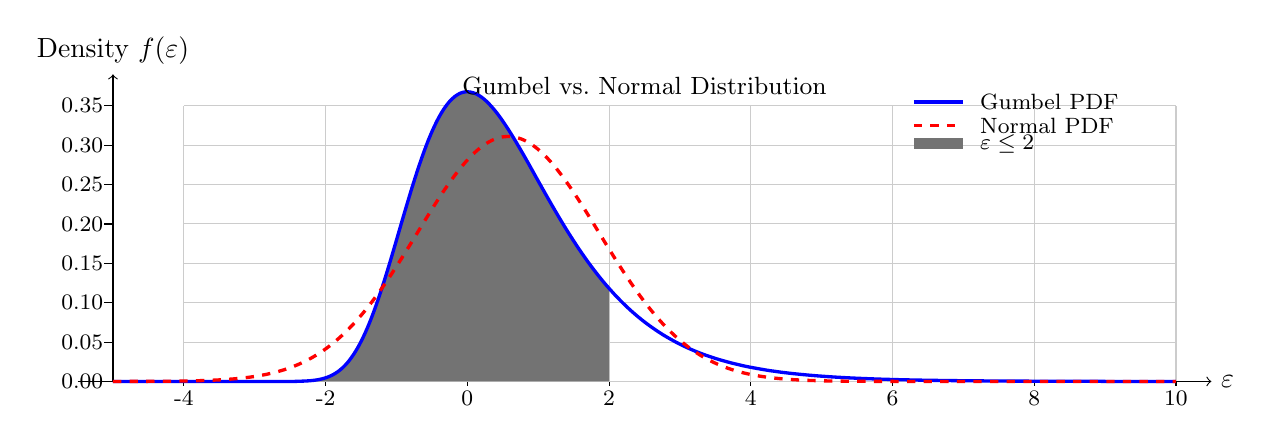
\begin{tikzpicture}[x=0.9cm,y=10cm]
  % axes
  \draw[->] (-5.5,0) -- (10.5,0) node[right] {$\varepsilon$};
  \draw[->] (-5,0) -- (-5,0.39) node[above] {Density $f(\varepsilon)$};

  % x ticks
  \foreach \x in {-4,-2,0,2,4,6,8,10}{
    \draw (\x,0) -- (\x,-0.006);
    \node[below,font=\footnotesize] at (\x,0) {\x};
  }

  % y ticks
  \foreach \y in {0.00,0.05,0.10,0.15,0.20,0.25,0.30,0.35}{
    \draw (-5,\y) -- (-5.12,\y);
    \node[left,font=\footnotesize] at (-5,\y) {\y};
  }

  % grid
  \draw[gray!40, thin] (-4,0) grid[xstep=2,ystep=0.05] (10,0.35);

  % shaded area
  \fill[black!55]
    plot[smooth,domain=-5:2,samples=120]
      (\x,{exp(-(\x + exp(-\x)))})
    -- (2,0) -- (-5,0) -- cycle;

  % Gumbel curve
  \draw[blue, very thick]
    plot[smooth,domain=-5:10,samples=200]
      (\x,{exp(-(\x + exp(-\x)))});

  % Normal distribution (mu=0.5772, sigma=pi/sqrt(6)=1.2826) to match Gumbel mean & variance
  \draw[red, very thick, dashed]
    plot[smooth,domain=-5:10,samples=200]
      (\x,{exp(-0.5*((\x - 0.5772)/1.2826)^2) / (1.2826*2.5066)});

  % title
  \node[font=\small] at (2.5,0.375)
    {Gumbel vs.\ Normal Distribution};

  % legend
  \draw[blue, very thick] (6.3,0.355) -- (7.0,0.355);
  \node[right,font=\footnotesize] at (7.1,0.355) {Gumbel PDF};

  \draw[red, very thick, dashed] (6.3,0.325) -- (7.0,0.325);
  \node[right,font=\footnotesize] at (7.1,0.325) {Normal PDF};

  \fill[black!55] (6.3,0.295) rectangle (7.0,0.309);
  \node[right,font=\footnotesize] at (7.1,0.302) {$\varepsilon \le 2$};
\end{tikzpicture}